This chapter addresses the software architecture.
It starts by setting up the IOb-Soc and configuring the firmware to allow execution of \textit{TwoLAME} encoding algorithm. Then, software optimizations are done to run \textit{TwoLAME} in FPGA. 
At the end, a detailed profiling analysis defines which part of the \textit{TwoLAME} software requires hardware acceleration.

Knowing beforehand that \textit{TwoLAME} uses floating-point arithmetic (FP)~\cite{floatingpoint}, porting the software to PICORV32 CPU would not be the best option, due to its fixed-point arithmetic limitation. Therefore, the ideal option is porting \textit{TwoLAME} to \textbf{VEXRISCV} (RV32IM) CPU, since it includes a floating-point unit (FPU)~\cite{fpu}.
In this process, the first step was removing the \textit{PICORV32} from the IOb-SoC and adding the VEXRISCV as the only CPU. This was straightforward, as \textit{VEXRISCV} was previously implemented and tested by \textit{IObundle, Lda}. Apart from adding the submodule to IOb-SoC's repository, some paths were changed to allow the correct compilation of the CPU. Interrupt signals were also added to the system data bus, such as \textit{timerInterrupt}, \textit{softwareInterrupt}, and \textit{externalInterrupt}.

\subsection{Audio testing}

Before porting the software, the \textit{TwoLAME} itself had to be verified. This verification was just in a practical way since this open-source software was already tested and approved by other users in various systems, with positive feedback. Considering this, the verification consisted of listening to an original audio file and the corresponding encoded file, produced by \textit{TwoLAME}.

%For testing purposes
To do so, four audio files were initially generated with \textit{Audacity} software. This is free open-source audio software, compatible with GNU/Linux (current working environment), and capable of multi-track audio editing and recording.
There are some reasons for having more than one testing file, preferably with different characteristics. One of them is the number of frames, which varies depending on several factors, including the audio codec being used, the settings or parameters selected for encoding, and the duration of the audio being processed (the easiest to notice). Another reason is the ability to check if the encoding software behaves the same way for different specifications, which is a crucial point as the main goal of the intended IP core is to allow real-time encoding.

Thus, the first generated file was \textit{short.wav}, using the \textit{Generate Tone} option in \textit{Audacity}. This mono audio has a sine waveform, 44.1KHz sampling rate, 16 bits per sample, and a size of 27KB (the smallest audio file in the repository).

The second generated file was \textit{long.wav}, using the \textit{Generate Rhythm Track} option configured with \textit{Metronome Tick} beat sound in \textit{Audacity}. This mono audio has a 44.1KHz sampling rate, 16 bits per sample, and a size of 683KB.

The third generated file was \textit{noise.wav}, using the \textit{Generate Noise} option configured with \textit{White} noise type in \textit{Audacity}. This audio has a 44.1KHz sampling rate, 16 bits per sample, a size of 529KB and, unlike the previous ones, it is stereo. The mono default track was duplicated, with one being distributed 100\% to the Left and the other being distributed 100\% to the Right (\textit{panning effect}).

The fourth and last generated file was \textit{vivaldi.wav}. This file was not generated from scratch in \textit{Audacity}. Instead, it was simply converted to WAV format. The original file, entitled 'Vivaldi - Spring', was downloaded from the Internet (for free) and opened on \textit{Audacity}. After that, the track was reduced to the initial 4 seconds and exported as WAV. What motivated the use of this file was the recognized quality and complexity of Vivaldi's songs.

With four audio files available at the repository, it was possible to verify the \textit{TwoLAME} software. Using a standard \textit{automake} process, composed of \textit{./configure}, \textit{make}, and \textit{make install} commands, \textit{TwoLAME} was successfully installed. Then, by simply typing \textit{stwolame} followed by the input file name, white space, and the output file name (the one desired), the software would run and produce an MP2-encoded version of the original file.
It is important to mention that both input and output file names should include the file extension. For this work, the relevant extensions are '.wav' as input and '.mp2' as output.
From executing \textit{stwolame short.wav short.mp2} command, it was verified that both the original and the encoded audio files sound the same (for a human listener). The same happened with the second and fourth files through a similar command. 
The third file is not audible, in the way that it was created just to verify proper correctness in terms of values produced. This is because white noise is the worst-case scenario for audio encoding, mainly due to its high requirements. \\


After testing the original \textit{TwoLAME} software, it was necessary to implement it in IOb-SoC. The porting of the software requires a front end, as the encoding process uses functions of \textit{libtwolame} (\textit{TwoLAME}'s library). 

\subsection{Firmware}

The front end should instantiate all the required functions to produce an MP2 audio. Considering this, the \textit{simplefrontend} example was taken from the \textit{TwoLAME} repository, improved, and implemented in \textit{firmware.c}.
%doesnt have a file system
To realize what modifications are necessary to run \textit{TwoLAME} in IOb-SoC, figure \ref{newpseudo} shows the pseudo code for the \textit{main()} function in \textit{firmware.c}.

\begin{figure}[H]
\centerline{\fbox{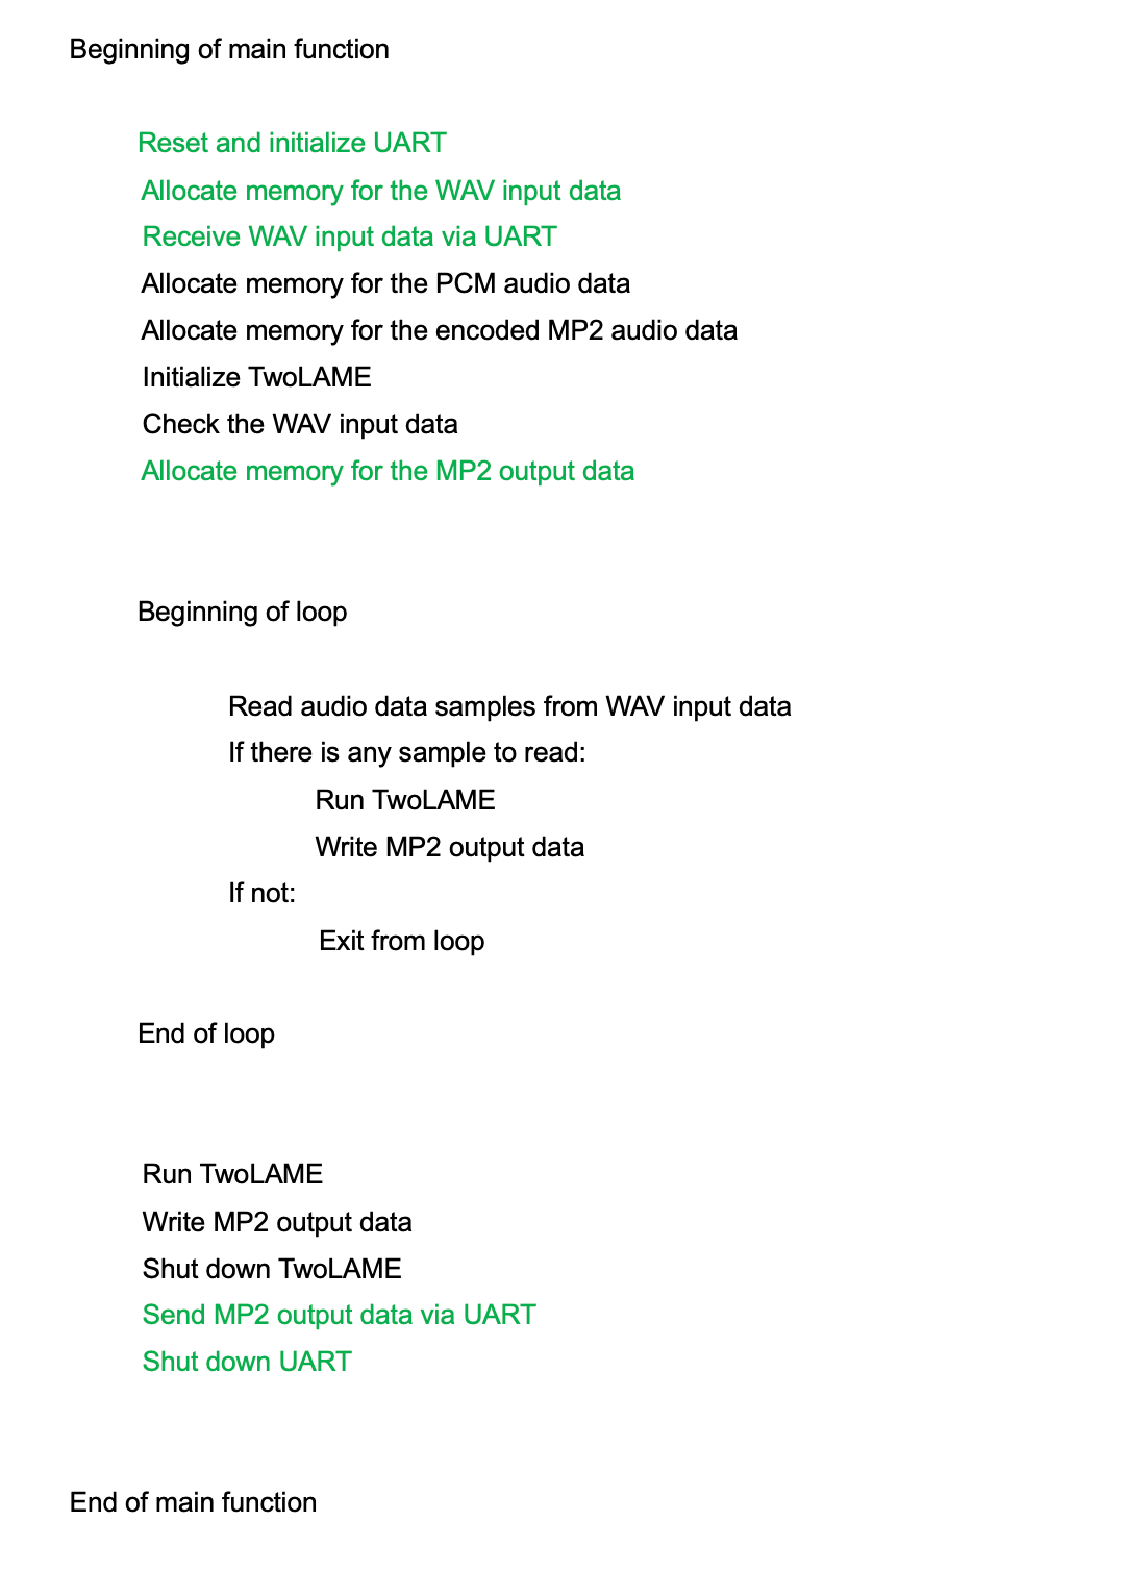
\includegraphics[width=0.80\linewidth]{newpseudo.pdf}}}
\caption{New \textit{firmware.c} pseudo code.}
\label{newpseudo}
\end{figure}

The first difference in \textit{main()} is the usage of \textit{uart\_init}, which resets \textit{IObundle, Lda}’s UART peripheral and sets its division factor. This peripheral is needed to transmit data between IOb-UART and IOb-Console. 
There are also two additional memory allocations for the input and output data. These operations are done through \textit{malloc} using unsigned char type because UART peripheral does transmit one byte at a time.
After allocating memory, the input audio data is received via UART in \textit{uart\_recvfile}. The function receives the path as an argument, which is defined as \textit{test.wav}. This is a generic name since the input audio file is copied to the compiling directory as \textit{test.wav}.
The previous modifications were done because the IOb-SoC does not have an operating system or file system. For this reason, the \textit{fopen} function inside \textit{wave\_init} was removed. Furthermore, in each iteration of the \textit{while} loop, a chunk of input data is read from the input data using \textit{fread}. Since this function, present in \textit{wave\_get\_samples}, also requires a file system, there should be some process to increment the pointer to the input data, so that \textit{fread} can be removed. This is achieved by decrementing a global variable (unread\_data) based on the number of samples read in each loop iteration. In addition, since the \textit{pcmaudio} buffer should contain short integers, there is a process inside \textit{wave\_get\_samples} that converts every two characters into a single short integer. This is done by concatenating two characters, with the first one shifted left eight positions.

Nonetheless, not only the input audio data is received via UART but also the output audio data is sent via UART. Thus, the \textit{fwrite} functions were also removed from \textit{main}.
More precisely, there was one situation inside the \textit{while} loop and another after the loop, with both \textit{memcpy} insertions being responsible for writing the MP2 output data, replacing \textit{fwrite} calls. An important detail about this modification comes with the pointer to the output data. Just like in \textit{wave\_get\_samples}, there should be a process to increment the pointer to the output data, so that the new data does not overwrite previous data. This process is based on the number of frames encoded in each loop iteration, specifically inside \textit{\textit{TwoLAME}\_encode\_buffer\_interleaved} function.
One of the last modifications in \textit{main} consists of sending the output data via UART in \textit{uart\_sendfile}. The function receives the path as an argument, which is defined as ’../../encoded.mp2’. This way, the output audio file is copied to the main repository directory as \textit{encoded.mp2}.
Afterward, the UART transmission is closed through \textit{uart\_finish}, and the program returns.

Apart from main(), some header files were included in \textit{firmware.c}, related to both the IOb-SoC system and \textit{TwoLAME} front end. Two macros were also defined, AUDIOBUFSIZE as 2304 and MP2BUFSIZE as 4096. These variables specify the size of input and output buffers, respectively, which in practice represent the chunk of data encoded each time (the number of frames encoded). Therefore, the number of frames can be altered by changing both variables on the same scale. As it stands, the \textit{TwoLAME} encodes one frame at a time.


\subsection{Optimization}

With the \textit{TwoLAME} already implemented in firmware.c, it is possible to emulate the program, by running it on a PC. It is also possible to simulate its execution on a PC. However, the major interest is in running \textit{TwoLAME} in FPGA, as the goal is to encode MP2 audio in real time. Considering this, some basic software improvements were done before evaluating the performance in FPGA.

The first change in \textit{libtwolame} was the software precision. In \textit{comon.h}, there is a macro for FLOAT that was initially defined as \textit{double}, but it was changed to \textit{float}. One reason for this is the fact that \textit{TwoLAME} should be faster rather than more accurate, without compromising the encoded audio quality. The other reason was IOb-SoC does not support double precision, since it contains floating-point units with single precision, exclusively. Apart from altering the macro, one function in \textit{subband.c} was also changed. The original code contained \textit{modf}, a function that belongs to \textit{math.h} and requires double precision. Therefore, it was substituted by \textit{modff}, which has the same functionality (returns the fractional part) but uses single precision.

The second change was more strategic, as it involved a more careful analysis of the encoding software. It is known that trigonometric functions are computationally complex, and \textit{TwoLAME}, as an audio-processing software, requires different mathematical functions. For this reason, some math functions were removed and substituted by tables, wherever it was possible. To evaluate this possibility, the \textit{TwoLAME} was emulated on a PC, and compiled with different test files.

The first case was \textit{psycho\_3\_powerdensityspectrum}, in \textit{psycho\_3.c}. In this function, there was a \textit{log10} operation inside a \textit{i} loop, with \textit{i} ranging from 1 to 512 (HBLKSIZE-1). Since the \textit{log10} operation was performed based on \textit{energy[i]}, the solution was creating a table with 512 positions, so that \textit{energy[i]} determines the index that should be accessed from the table. To be linear access, \textit{energy[i]} has to be multiplied by 1000 and converted to an integer. Since it is guaranteed that in the \textit{else} condition the array value is always positive, a condition was added to upper limit the index of the log10 table (511 is the maximum index). With this, and noticing the multiplication by 10 (of log10) in the original code, the \textit{tablog10\_psycho\_3\_powerdensityspectrum} was created by calculating $LOG10(x/10000)$ in an excel sheet, with \textit{x} ranging from 0 and 511. It was then copied and defined in \textit{psycho\_3.c}, with a change in index 0. Since \textit{log10(0)=-inf}, the first index in the table was defined as -40 (the same value as index 1).

\begin{comment}
\begin{figure}[H]
\centerline{\fbox{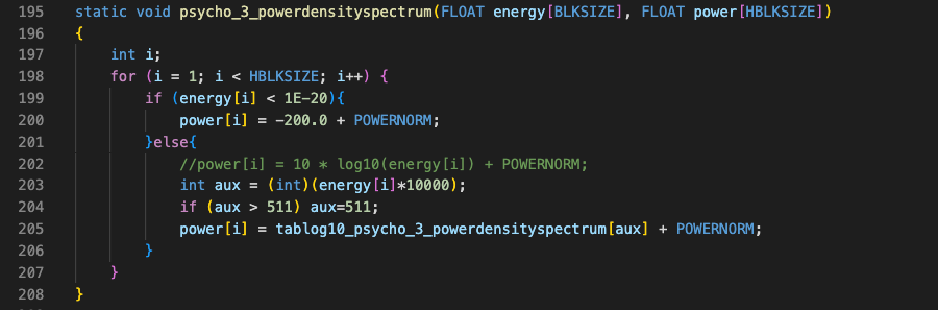
\includegraphics[width=0.80\linewidth]{powerdensityspectrum.pdf}}}
\caption{\textit{psycho\_3\_powerdensityspectrum} function.}
\label{powerdensityspectrum}
\end{figure}
\end{comment}

%\vspace{1cm}

The second case was \textit{psycho\_3\_init\_add\_db}, also in \textit{psycho\_3.c}. In this function, there were both \textit{pow} and \textit{log10} operations inside a \textit{i} loop, with \textit{i} ranging from 0 to 999 (DBTAB-1). However, this case was straightforward to solve, since the result produced in each iteration does not depend on any input data. Considering this, the \textit{tablog10\_psycho\_3\_init\_add\_db} was created by calculating the whole expression in an excel sheet, with \textit{x} ranging from 0 to 99.9 ($x=i/10.0$).

\begin{comment}
\begin{figure}[H]
\centerline{\fbox{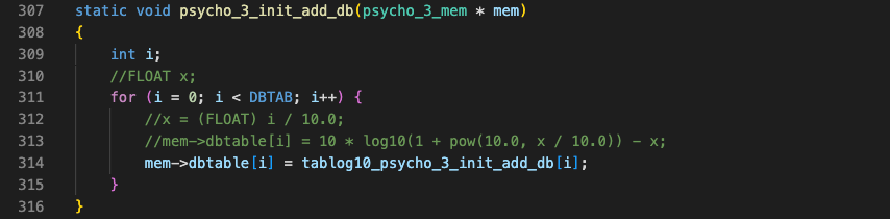
\includegraphics[width=0.80\linewidth]{init.pdf}}}
\caption{\textit{psycho\_3\_init\_add\_db} function.}
\label{init}
\end{figure}
\end{comment}

%\vspace{1cm}

The third case was \textit{psycho\_3\_spl}, in \textit{psycho\_3.c}. In this function, there was a \textit{log10} operation inside a \textit{i} loop, with \textit{i} ranging from 0 to 31 (SBLIMIT-1). Since the \textit{log10} operation was performed based on \textit{scale[i]} and its value was never higher than 20000 (after being multiplied by 32768), the solution was creating a table with 2000 positions, so that \textit{scale[i]} determines the index that should be accessed from the table. 
To be linear access, \textit{scale[i]} has to be multiplied by 3276.8 and converted to an integer. Since it is guaranteed that the array value is always positive, a condition was added to limit the index of the log10 table (1999 is the maximum index). With this, and noticing the multiplication by 20 followed by the subtraction by 10 (of log10) in the original code, the \textit{tablog10\_psycho\_3\_spl} was created by calculating $20\times log10(x\times 10)-10$ in an excel sheet, with \textit{x} ranging from 0 and 1999. It was then copied and defined in \textit{psycho\_3.c}.

\begin{comment}
\begin{figure}[H]
\centerline{\fbox{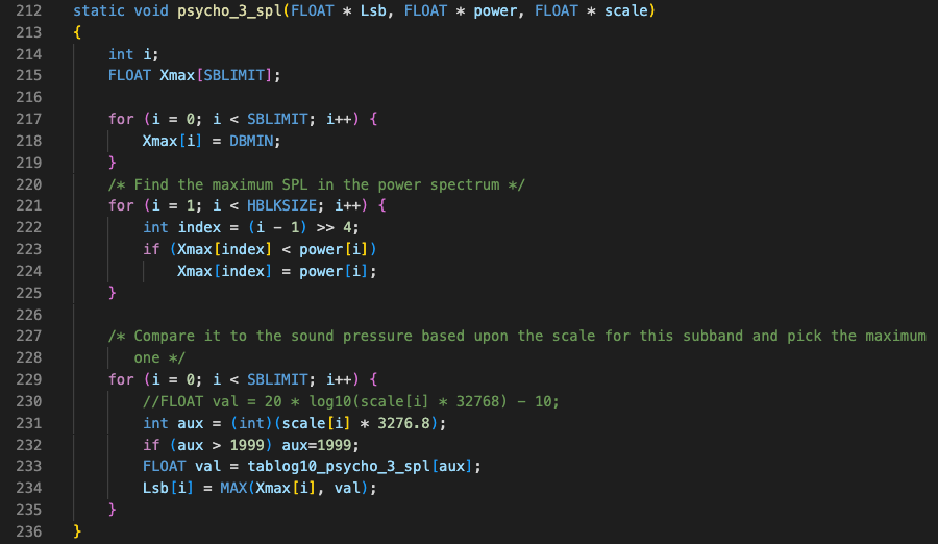
\includegraphics[width=0.80\linewidth]{spl.pdf}}}
\caption{\textit{psycho\_3\_spl} function.}
\label{spl}
\end{figure}

\vspace{1cm}
\end{comment}

The fourth case was \textit{psycho\_3\_fft}, in \textit{psycho\_3.c} too. In this function, there was a \textit{pow} operation and also a \textit{cos} operation inside a \textit{i} loop, with \textit{i} ranging from 0 to 1023 (BLKSIZE-1). This case was straightforward to solve since the result produced in each iteration does not depend on any input data. Considering this, the \textit{tabcos\_psycho\_3\_fft} was created by calculating both expressions in an Excel sheet, with \textit{x} ranging from 0 to 1023.

\begin{comment}
\begin{figure}[H]
\centerline{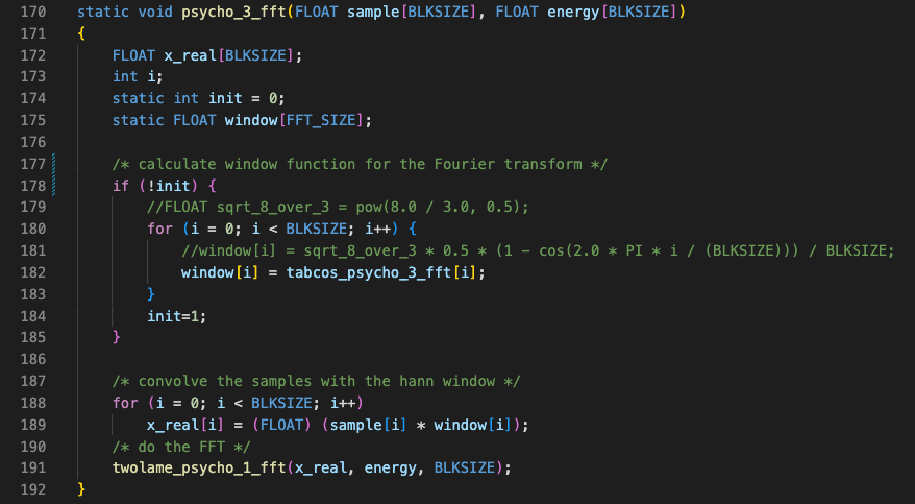
\includegraphics[width=0.80\linewidth]{fft.pdf}}
\caption{\textit{psycho\_3\_fft} function.}
\label{fft}
\end{figure}

\vspace{1cm}
\end{comment}

The fifth and last case was \textit{create\_dct\_matrix}, in \textit{subband.c}. In this function, there was a \textit{cos} operation inside a nested loop, with \textit{i} ranging from 0 to 15 and \textit{k} ranging from 0 to 31. This case was also straightforward to solve since the result produced in each iteration does not depend on any input data. Considering this, the \textit{tabcos\_create\_dct\_matrix} was created by calculating the whole expression in an Excel sheet, with \textit{aux} ranging from 0 to 511 ($16 \times 32$).

\begin{comment}
\begin{figure}[H]
\centerline{\fbox{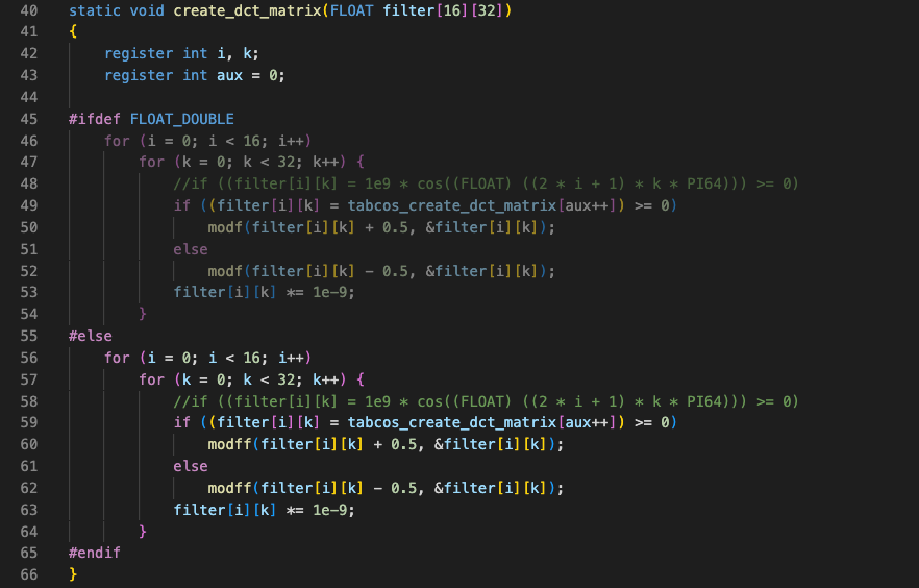
\includegraphics[width=0.80\linewidth]{dct.pdf}}}
\caption{\textit{create\_dct\_matrix} function.}
\label{dct}
\end{figure}

\vspace{1cm}
\end{comment}

The third and last change in \textit{libtwolame} was related to memory.
Initially, there was a memory allocation for \textit{bit\_stream} struct in \textit{twolame\_buffer\_init}, called from \textit{twolame\_encode\_buffer\_interleaved} function. Since this function executes in every \textit{while} loop iteration, in \textit{firmware.c}, the memory allocation was also performed many times.
Therefore, the \textit{TWOLAME\_MALLOC} of \textit{bit\_stream} struct was moved to the \textit{main} function, meaning that it executes just once before the encoding process starts.
In addition, the \textit{TWOLAME\_FREE} in \textit{twolame\_buffer\_deinit}, called from \textit{twolame\_encode\_buffer\_interleaved}, was removed and, consequently, added to \textit{main}.

%grep -r 'tab' *

%\subsection{FPGA}

With basic software optimizations already implemented, it is desired to measure the execution time of the \textit{TwoLAME} software for different input data. This requires different memory management since the FPGA has memory space available, and so allocating memory during program execution is not ideal, except in special cases. Considering this, a macro called \textit{PC\_EMUL\_RUN} is defined to control each memory allocation, through an if directive. In the first case when the program is emulated on PC, \textit{PC\_EMUL\_RUN} should be defined. In a second case when the program runs in FPGA, \textit{PC\_EMUL\_RUN} should not be defined.
Focusing on the second case, the memory space available starts at \textit{DATA\_BASE\_ADDR}. This macro defines the base address based on IOb-SoC macros from \textit{config.mk}, the IOb-SoC configuration script (explained in the next section).
In \textit{main()}, the first example is \textit{recvfile\_ch} pointer, which represents where the input data is stored in memory. As it is the first, it should be equal to \textit{DATA\_BASE\_ADDR}.
The second example is \textit{pcmaudio} pointer, which represents where the input data buffer is stored. As it is the second, it should be equal to DATA\_BASE\_ADDR + recv\_file\_size (the size of the input file).
The third example is \textit{mp2buffer} pointer, which represents where the encoded data buffer is stored. It should be equal to $pcmaudio + AUDIObUFSIZE*sizeof(short)$ (the second pointer plus the size of the input data buffer).
The fourth example is \textit{mybs} pointer, which represents where the bit\_stream struct is stored. It should be equal to $mp2buffer + MP2BUFSIZE*sizeof(unsigned char)$ (the third pointer plus the size of the encoded data buffer).
The fifth and last example is \textit{outfile} pointer, which represents where the encoded MP2 data is stored. It should be equal to $mybs + sizeof(bit\_stream)$ (the fourth pointer plus the size of the \textit{bit\_stream} struct).
In addition, the \textit{free()} functions were also inserted in a \textit{\#ifdef PC\_EMUL\_RUN} directive, since the function should only be called when the memory is dynamically allocated. \\

\subsection{Profiling}

With everything set up, the last implementation in the software architecture was \textbf{profiling}. This process is a form of dynamic program analysis that can measure different variables, like memory space or time complexity. In this case, it was used to measure the duration of each function.
To do so, an eight component was added to IOb-SoC, the \textbf{TIMER}. This peripheral is a 64-bit hardware timer, equipped with reset, enable, and reading functions. It includes a software driver and an example C application, which helps understand how it works. 
Similarly to the other components, the TIMER is tracked by a \textit{GitHub} repository (forked from \textit{IObundle, Lda}), integrating the IOb-SoC as a submodule. This component was previously implemented and tested by \textit{IObundle, Lda} as well. In addition, some paths were added to allow correct compilation.

With this, IOb-SoC was ready for profiling. The process consisted of three phases, with the first phase being a more high-level approach. 
This phase was simple since only the function calls directly made from \textit{main()} were considered. The timer was first initialized through \textit{timer\_init(TIMER\_BASE)} function. Then, a \textit{elapsed\_time} integer array of size 50 was declared and set with zero. In the profiling itself, some basic operations were used for each function call. Immediately before a function call, \textit{timer\_time\_ms()} is invoked, returning the current time in ms which is then stored in \textit{start\_elapse\_time} variable as an unsigned integer. Immediately after a function call, \textit{timer\_time\_ms()} is invoked again, returning the current time in ms which is then stored in \textit{end\_elapse\_time} variable as an unsigned integer as well. Then, the difference between both variables is calculated and stored in a certain index of \textit{elapsed\_time} array (one index for each function call). 
By doing this, 13 functions were included in the first phase of \textit{TwoLAME} profiling. At the end of \textit{main()}, every position of the array is printed, showing how many ms each function call took. The printing does not influence the profiling, as it is done after the last function measurement. Another interesting detail is that both \textit{uart\_recvfile} and \textit{uart\_sendfile} functions are excluded from the profiling, which is correct since they perform data transfers that are not part of the \textit{TwoLAME}.
Table \ref{profiling1} shows the first phase of the profiling for all input files.

\begin{table}[H]
    \centering
    \begin{tabular}{c|c|c|c|c|}
    \cline{2-5}
    \multicolumn{1}{c|}{}  & \multicolumn{4}{c|}{\textbf{Input file}} \\
    \cline{2-5}
     & short.wav & long.wav & noise.wav & vivaldi.wav \\
    \hline
    \multicolumn{1}{|c|}{\textit{TwoLAME}\_init()}  & 3 & 2 & 3 & 0 \\ 
    \hline
    \multicolumn{1}{|c|}{wave\_init()}  & 0 & 0 & 0 & 0 \\ 
    \hline
    \multicolumn{1}{|c|}{\textit{TwoLAME}\_set\_num\_channels()}   & 0 & 0 & 0 & 0 \\ 
    \hline
    \multicolumn{1}{|c|}{\textit{TwoLAME}\_set\_in\_samplerate()}   & 0 & 0 & 0 & 0 \\ 
    \hline
    \multicolumn{1}{|c|}{\textit{TwoLAME}\_set\_bitrate()}   & 0 & 0 & 0 & 0 \\ 
    \hline
    \multicolumn{1}{|c|}{\textit{TwoLAME}\_init\_params()}   & 11 & 11 & 11 & 11 \\ 
    \hline
    \multicolumn{1}{|c|}{wave\_get\_samples()}   & 4 & 126 & 89 & 135 \\ 
    \hline
    \multicolumn{1}{|c|}{\textit{TwoLAME}\_encode\_buffer\_interleaved()}   & 1510 & 24345 & 19820 & 26010 \\ 
    \hline
    \multicolumn{1}{|c|}{memcpy()}  & 2 & 59 & 19 & 32 \\ 
    \hline
    \multicolumn{1}{|c|}{\textit{TwoLAME}\_encode\_flush()}   & 79 & 80 & 185 & 155 \\ 
    \hline
    \multicolumn{1}{|c|}{memcpy()}  & 0 & 0 & 0 & 0 \\ 
    \hline
    \multicolumn{1}{|c|}{\textit{TwoLAME}\_close()}   & 0 & 0 & 0 & 1 \\ 
    \hline
    \multicolumn{1}{|c|}{\textbf{\textit{TwoLAME} total}}  & 1614 & 24719 & 20210 & 26467 \\ 
    \hline
    \end{tabular}
    \caption{Execution time for all input files [ms].}
    \label{profiling1}
\end{table}

\vspace{1cm}


The previous table shows that \textit{twolame\_encode\_buffer\_interleaved} occupies most of the execution time, which is expected as it is responsible for the encoding, calling many other \textit{TwoLAME} functions. Nonetheless, this information is not enough, mainly because developing hardware to accelerate the whole function would be an extremely difficult task.
By analyzing \textit{twolame\_encode\_buffer\_interleaved}, it is noticeable that the relevant operation inside the function is \textit{encode\_frame()}, as all the other operations are basic.
Considering this, the second phase of profiling includes all function calls inside \textit{encode\_frame}. 
This phase was similar to the previous one in terms of methodology. The only differences were the usage of the \textit{elapsed\_time\_\textit{TwoLAME}} array, which was declared and set to 0 in \textit{main()} and passed as an argument to \textit{twolame\_encode\_buffer\_interleaved} and \textit{encode\_frame()}, consecutively. The variables that store the time values are also different, being \textit{start\_elapse\_time\_twolame} and \textit{end\_elapse\_time\_twolame}, declared in \textit{twolame.c} as global unsigned integers.
By doing this, 23 functions were included in the second phase of \textit{TwoLAME} profiling. It was not 23 functions but 23 blocks of code from \textit{encode\_frame()}, because apart from the \textit{libtwolame} functions, there is additional code that has to be included for correct measurements, like if conditions and \textit{for} loops.
At the end of \textit{main()}, every position of the array is printed, showing how many ms each part of \textit{encode\_frame()} took. 
Table \ref{profiling2} shows the second phase of the profiling for all input files.

\begin{table}[H]
    \centering
    \begin{tabular}{|c|c|c|c|c|c|}
    \cline{3-6}
    \multicolumn{2}{c|}{}  & \multicolumn{4}{c|}{\textbf{Input file}} \\
    \cline{3-6}
    \multicolumn{2}{c|}{} & \textit{short.wav} & \textit{long.wav} & \textit{noise.wav} & \textit{vivaldi.wav} \\
    \cline{1-6}
   \multirow{23}{*}{\parbox{2.5cm}{\centering \textbf{\textit{TwoLAME}} \\ \textbf{\_encode} \\ \textbf{\_buffer} \\ \textbf{\_interleaved()}}}  & \multicolumn{1}{c|}{\textit{scale\_and\_mix\_samples}}  & 0 & 9 & 5 & 3 \\ 
    \cline{2-6}
    & \multicolumn{1}{c|}{\textit{twolame\_buffer\_sstell}} & 3 & 139 & 52 & 78 \\ 
    \cline{2-6}
    & \multicolumn{1}{c|}{\textit{twolame\_available\_bits}} & 0 & 16 & 7 & 8  \\ 
    \cline{2-6}
    & \multicolumn{1}{c|}{\textit{twolame\_window\_filter\_subband}} & 141  & 3487 & 2590 & 3662  \\ 
    \cline{2-6}
    & \multicolumn{1}{c|}{\textit{twolame\_scalefactor\_calc}} & 7 & 172 & 142 &  201  \\ 
    \cline{2-6}
    & \multicolumn{1}{c|}{\textit{twolame\_find\_sf\_max}} & 0  & 13 & 3 & 6   \\ 
    \cline{2-6}
    & \multicolumn{1}{c|}{\textit{twolame\_scalefactor\_calc}} & 0  & 5 & 6 & 4  \\ 
    \cline{2-6}
     & \multicolumn{1}{c|}{\textit{twolame\_psycho\_3}} & 1377  & 19062 & 16222 &  20829 \\ 
    \cline{2-6}
    & \multicolumn{1}{c|}{\textit{twolame\_sf\_transmission\_pattern}} & 0 & 17 & 8 &  10 \\ 
    \cline{2-6}
    & \multicolumn{1}{c|}{\textit{twolame\_main\_bit\_allocation}} & 16  & 424 & 343 & 485  \\ 
    \cline{2-6}
    & \multicolumn{1}{c|}{\textit{twolame\_write\_header}} & 2 & 12 & 7 &  7 \\
    \cline{2-6}
    & \multicolumn{1}{c|}{\textit{buffer\_putbits}} & 0 & 4 & 1 & 4  \\
    \cline{2-6}
    & \multicolumn{1}{c|}{\textit{twolame\_write\_bit\_alloc}} & 0 & 11 & 11 &  17 \\
    \cline{2-6}
    & \multicolumn{1}{c|}{\textit{twolame\_write\_scalefactors}} & 1 & 22 & 20 & 27 \\
    \cline{2-6}
    & \multicolumn{1}{c|}{\textit{twolame\_subband\_quantization}} & 21 & 503 & 346 & 488 \\
    \cline{2-6}
    & \multicolumn{1}{c|}{\textit{twolame\_write\_samples}} & 12 & 306 & 149 & 210 \\
    \cline{2-6}
    & \multicolumn{1}{c|}{\textit{buffer\_put1bit}} & 0 & 10 & 4 & 2 \\
    \cline{2-6}
    & \multicolumn{1}{c|}{\textit{buffer\_putbits}} & 0 & 5 & 4 & 2 \\
    \cline{2-6}
    & \multicolumn{1}{c|}{\textit{twolame\_dab\_crc\_calc}} & 0 & 9 & 3 &  3 \\
    \cline{2-6}
    & \multicolumn{1}{c|}{\textit{buffer\_put1bit}} & 0 & 3 & 0 &  0 \\
    \cline{2-6}
    & \multicolumn{1}{c|}{\textit{twolame\_buffer\_sstell}} & 0 & 1 & 0 & 1  \\
    \cline{2-6}
    & \multicolumn{1}{c|}{\textit{twolame\_do\_energy\_levels}} & 0 & 7 & 1 & 3  \\
    \cline{2-6}
    & \multicolumn{1}{c|}{\textit{twolame\_crc\_writeheader}} & 0 & 3 & 1 &  2  \\ 
    \hline
    \multicolumn{2}{|c|}{\textbf{\textit{TwoLAME} total}}  & 1614 & 24719 & 20210 & 26467 \\ 
    \hline
    \end{tabular}
    \caption{Execution time for all input files [ms].}
    \label{profiling2}
\end{table}

\vspace{1cm}

The previous table shows that the eight block of \textit{encode\_frame()} occupies most of the execution time, which includes two nested loops (executed depending on \textit{if} conditions) and a switch case. The nested loops perform simple operations, so they are not relevant. The switch case calls a certain function depending on the switch condition. However, after inspecting \textit{glopts->psymodel} condition it is perceptible that case 3 is always selected, calling \textit{twolame\_psycho\_3}. Nevertheless, this information is still not enough. 
Looking at \textit{twolame\_psycho\_3}, there are many other \textit{libtwolame} functions inside it. Considering this, the third phase of profiling includes all function calls inside \textit{twolame\_psycho\_3}. 
This phase was also similar to the previous ones in terms of methodology. The only differences were the usage of the \textit{elapsed\_time\_psycho\_3} array, which was declared and set to 0 in \textit{main()} and passed as argument to \textit{twolame\_encode\_buffer\_interleaved}, \textit{encode\_frame()} and \textit{twolame\_psycho\_3}, consecutively. The variables that stored the time values were also different, being \textit{start\_elapse\_time\_psycho\_3} and \textit{end\_elapse\_time\_psycho\_3}, declared in \textit{twolame.c} as global unsigned integers.
By doing this, 13 blocks of code were included in the third phase of \textit{TwoLAME} profiling, with most of them being just functions.
At the end of \textit{main()}, every position of the array is printed, showing how many ms each block of \textit{twolame\_psycho\_3} took. 
Table \ref{profiling3} shows the third phase of the profiling for all input files.

\begin{table}[H]
    \centering
    \begin{tabular}{|c|c|c|c|c|c|}
    \cline{3-6}
    \multicolumn{2}{c|}{}  & \multicolumn{4}{c|}{\textbf{Input file}} \\
    \cline{3-6}
    \multicolumn{2}{c|}{} & short.wav & long.wav & noise.wav & vivaldi.wav \\
    \cline{1-6}
   \multirow{13}{*}{\parbox{2.3cm}{\centering \textbf{\textit{twolame\_} \\ \textit{psycho\_3}}}}  & \multicolumn{1}{c|}{twolame\_psycho\_3\_init}  & 635 & 642 & 635 & 635 \\ 
    \cline{2-6}
    & \multicolumn{1}{c|}{\textit{mem} $\rightarrow$ \textit{fft\_buf}} & 5 & 133 & 115 & 155 \\ 
    \cline{2-6}
    & \multicolumn{1}{c|}{\textit{mem} $\rightarrow$ \textit{fft\_buf}} &  6 &  117& 77 &  120 \\ 
    \cline{2-6}
    & \multicolumn{1}{c|}{\textit{psycho\_3\_fft}} & 47 & 1138 & 886 &  1253  \\ 
    \cline{2-6}
    & \multicolumn{1}{c|}{\textit{psycho\_3\_powerdensityspectrum}} & 40  & 1026 & 791 &  1115  \\ 
    \cline{2-6}
    & \multicolumn{1}{c|}{\textit{psycho\_3\_spl}} &  7 & 170 & 148 & 204  \\ 
    \cline{2-6}
     & \multicolumn{1}{c|}{\textit{psycho\_3\_tonal\_label}} &  7 & 153 & 258 & 173  \\ 
    \cline{2-6}
    & \multicolumn{1}{c|}{\textit{psycho\_3\_noise\_label}} & 8 & 220 & 167 & 235  \\ 
    \cline{2-6}
    & \multicolumn{1}{c|}{\textit{psycho\_3\_dump}} &  0 & 4 & 2 & 4  \\ 
    \cline{2-6}
    & \multicolumn{1}{c|}{\textit{psycho\_3\_decimation}} & 3 & 45 & 38 & 67   \\
    \cline{2-6}
    & \multicolumn{1}{c|}{\textit{psycho\_3\_threshold}} & 611 & 15168  & 12975 &  16684 \\
    \cline{2-6}
    & \multicolumn{1}{c|}{\textit{psycho\_3\_minimummasking}} & 0 & 23 & 14 & 29  \\ 
    \cline{2-6}
    & \multicolumn{1}{c|}{\textit{psycho\_3\_smr}} & 0 & 9 & 6 & 13  \\ 
    \hline
    \multicolumn{2}{|c|}{\textbf{\textit{TwoLAME} total}}  & 1614 & 24719 & 20210 & 26467 \\ 
    \hline
    \end{tabular}
    \caption{Execution time for all input files [ms].}
    \label{profiling3}
\end{table}

\vspace{1cm}

The previous table shows interesting information. First, it is noticeable that several functions have an insignificant execution time, compared to others. Second, it is clear that \textit{psycho\_3 function 11}, which is \textit{psycho\_3\_threshold}, occupies the biggest part of the program execution. For \textit{short.wav}, \textit{long.wav}, \textit{noise.wav} and \textit{vivaldi.wav}, this function corresponds to 37\%, 61\%, 64\% and 63\% of \textit{TwoLAME} execution time, respectively.
Therefore, \textit{psycho\_3\_threshold} should be the first function accelerated in Hardware.

%These functions have more specific names as we are going lower in abstraction.